

\documentclass{beamer}
\usepackage{swjtu}
\usepackage[style=ieee]{biblatex}
\setbeamertemplate{bibliography item}{\insertbiblabel}
\addbibresource{bibliography.bib}


\title{Convergence of an iterative nonlinear scheme
For denoising of piecewise constant images}
\subtitle{}
\author{Debwashis Borman}
\institute{Universität Göttingen}
\date{\today}

\begin{document}
%% Title page
%% Remove '[plain]' if you need a footline
\begin{frame}[plain]
    \titlepage
\end{frame}


%% TOC page
{
\begin{frame}
    \frametitle{Table of Contents}
    \tableofcontents
\end{frame}
}


%% Section One
\section{Introduction: some basic concepts}

%% Basic pages
\begin{frame}[t]{Image \& Denoising concepts}
 What is Pixel?
    \begin{itemize}
        \item Pixel:  Pixel, the fundamental building block of digital images smallest controllable element of a picture represented on a screen or digital display.
        Each pixel contains color information, usually represented as combinations of three primary colors: red, green, and blue (RGB). 
    \end{itemize}
    What is Resolution?
    \begin{itemize}
        \item The resolution of an image is measured in pixels and typically represented by the dimensions width x height. For instance, an image resolution of 1920 x 1080 means there are 1920 pixels in each row (width) and 1080 pixels in each column (height) of the image.
    \end{itemize}
\end{frame}

\begin{frame}[t]{Image \& Denoising concepts}
    \vspace{20pt}
    \begin{figure}
        \begin{columns}[onlytextwidth]
            \begin{column}{0.45\textwidth}
                \centering
                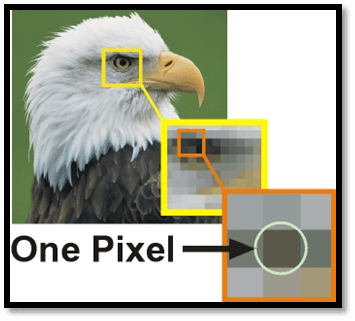
\includegraphics[width=\linewidth]{img/concept-of-pixel1.png}
               
                \label{fig:sub1}
            \end{column}
            \begin{column}{0.45\textwidth}
                \centering
                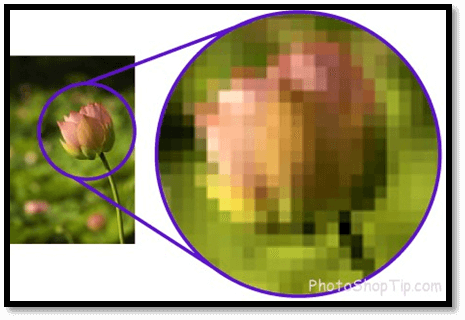
\includegraphics[width=\linewidth]{img/concept-of-pixel2.png}
               
                \label{fig:sub2}
            \end{column}
        \end{columns}
        \caption{Pixel visualization}
        \label{fig:images}
    \end{figure}
\end{frame}

\begin{frame}[plain]
    \frametitle{Pixel Representation in Images}
    \begin{itemize}
        \item \textbf{1-Channel Images (Grayscale)}: Each pixel is represented by a single intensity value, typically between 0 (black) and 255 (white). The pixel holds information about its intensity or brightness. 
        Example:
        \[
        \begin{pmatrix}
          50 & 100 & 150 \\
          200 & 255 & 0 \\
          80 & 120 & 90
        \end{pmatrix}
        \]
        \item \textbf{3-Channel Images (RGB)}: Each pixel is represented by three values, corresponding to the Red, Green, and Blue (RGB) channels. Each channel has intensity values ranging from 0 to 255. The pixel holds information about the intensity of red, green, and blue, which combine to form the pixel's final color. A 3-D matrix for RGB values:
        \[
        \begin{pmatrix}
          (255,0,0) & (0,255,0)\\
          (0,0,255) & (255,255,255)
        \end{pmatrix}
       
        \] 
    \end{itemize}
\end{frame}

\begin{frame}[t]{Image Noise}
 \frametitle{Image Noise}
    \begin{itemize}
        \item Image noise can be understood as the unwanted random variations or disturbances in an image that degrade its quality. Similar to the concept of noise in signal processing, where noise distorts the true signal, image noise interferes with the accurate representation or interpretation of an image. 
    \end{itemize}
    \begin{figure}
        \begin{columns}[onlytextwidth]
            \begin{column}{0.45\textwidth}
                \centering
                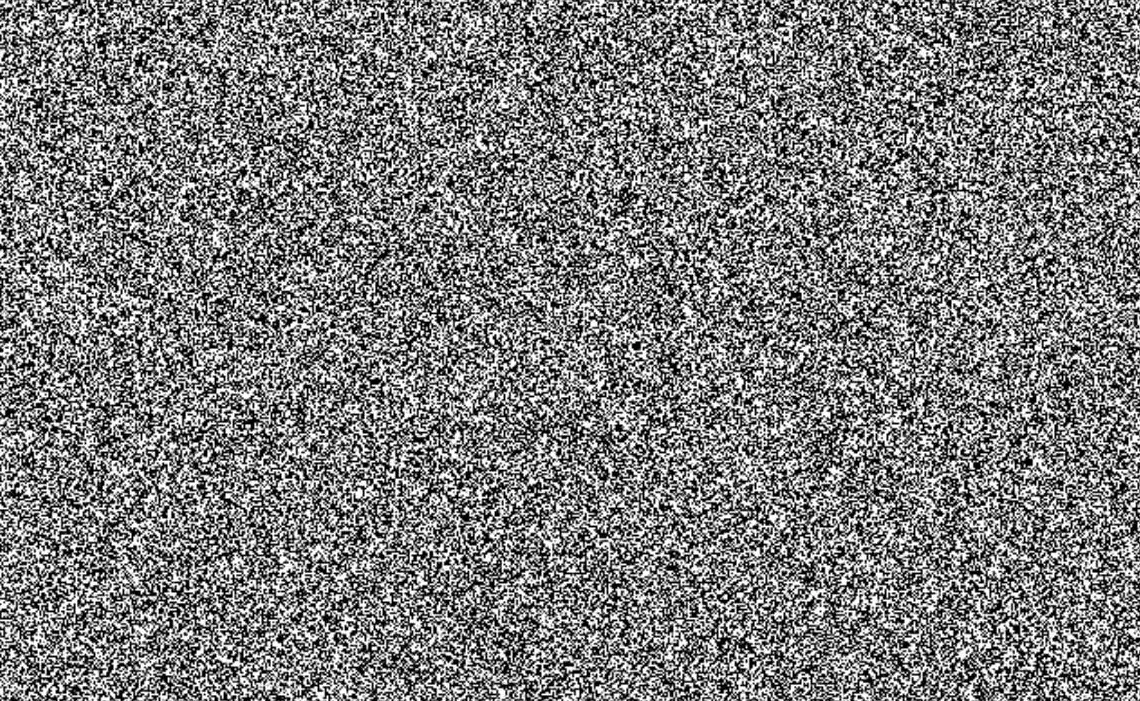
\includegraphics[width=\linewidth]{img/noise.png}
               % \caption{Typical white noise image}
               
                \label{fig:sub1}
            \end{column}
            \begin{column}{0.45\textwidth}
                \centering
                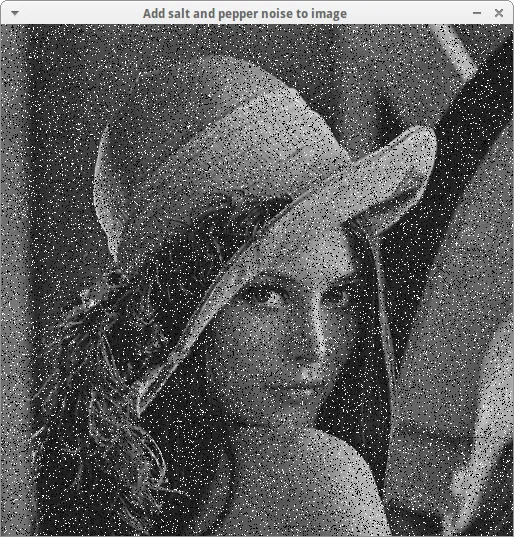
\includegraphics[width=.8\linewidth, scale=0.2]{img/salr_pepper.png}
               %\caption{Short noise}
                \label{fig:sub2}
            \end{column}
        \end{columns}
        \caption{Different Types of Noise}
        \label{fig:images}
    \end{figure}    
\end{frame}
\begin{frame}[plain]
\frametitle{Image Noise}
Types of Image Noise
    \begin{itemize}
        \item White Noise: In images, the pixels of a white noise image is assumed to be independent random variables with a uniform probability distribution over some set interval.
        
        \item Shot noise or Poisson noise is a type of noise which can be modeled by a Poisson process.
        \item Salt and Pepper Noise: This kind of noise if added to images will result in dark pixels in bright regions and bright pixels in dark regions, with a random frequency of occurrence.
    \end{itemize}
       \begin{figure}
        \begin{columns}[onlytextwidth]
            \begin{column}{0.3\textwidth}
                \centering
                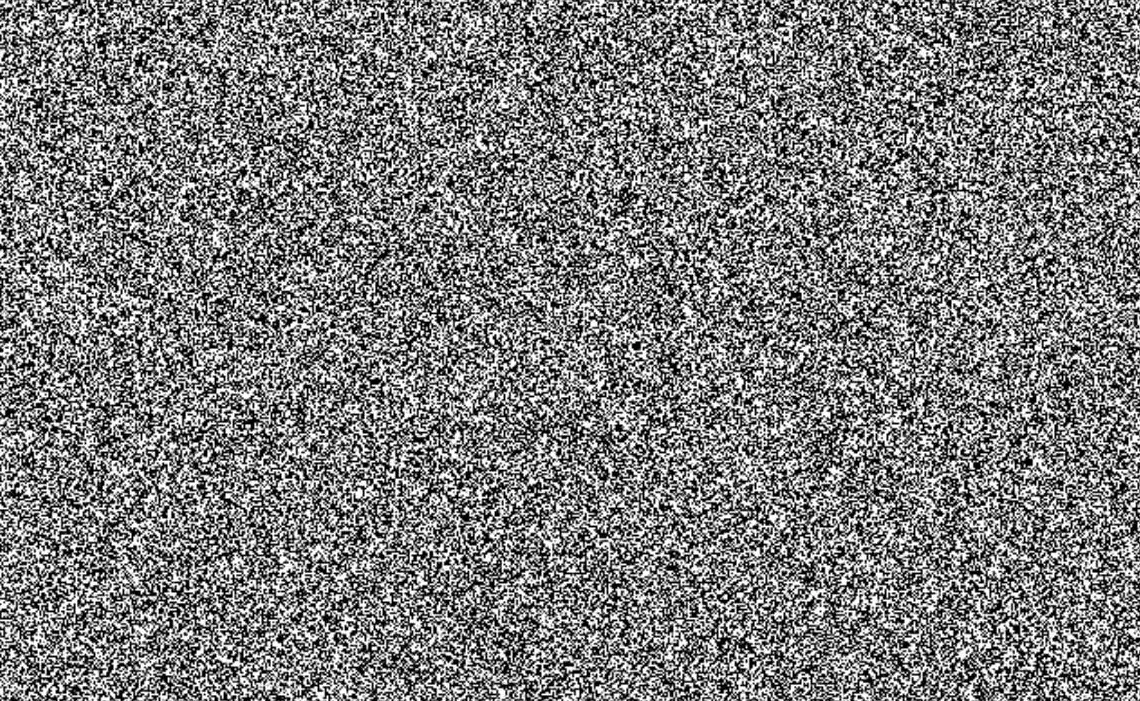
\includegraphics[width=.7\linewidth]{img/noise.png}
               \caption{white noise}
               
                \label{fig:sub1}
            \end{column}
            \begin{column}{0.3\textwidth}
                \centering
                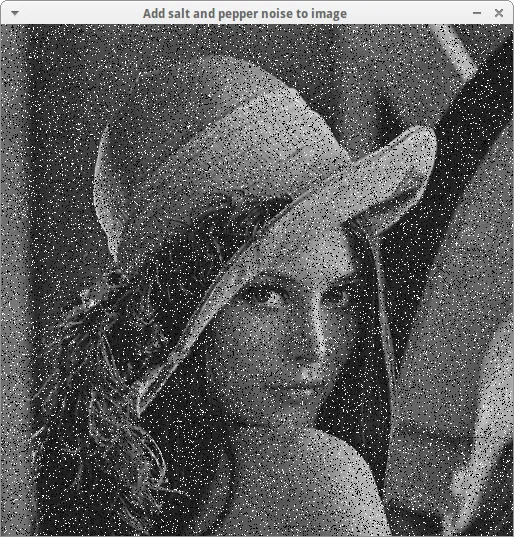
\includegraphics[width=.7\linewidth, scale=0.2]{img/salr_pepper.png}
               \caption{Salt and Pepper Noise}
                \label{fig:sub2}
            \end{column}
            \begin{column}{.3\textwidth}
                \centering
                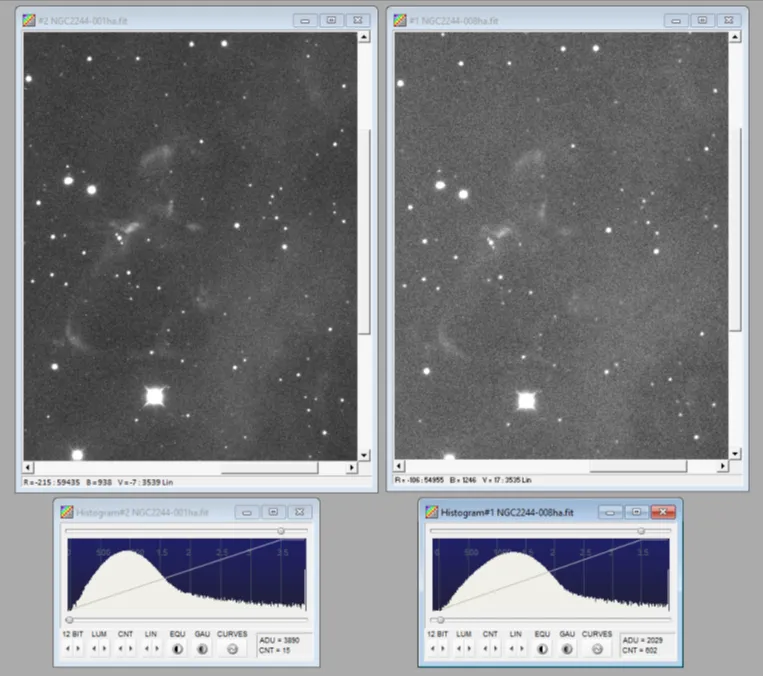
\includegraphics[width=.7\linewidth, scale=0.2]{img/short_noise.png}
               \caption{Short noise}
                \label{fig:sub2}
            \end{column}
        \end{columns}
       
        \label{fig:images}
    \end{figure}   
\end{frame}



\begin{frame}[plain]
\frametitle{Image Noise}
Common Sources of Image Noise
    \begin{itemize}
        \item Sensor Noise:  For example, in digital cameras, sensor noise can occur due to electronic disturbances or thermal noise within the camera's sensor.
        \item Environmental Factors: Poor lighting conditions can result in more noise in the image
        \item Transmission Errors: Lossy compression methods that discard some data to reduce the file size, or due to interference and loss in signal strength during wireless transmission.
    \end{itemize}
\end{frame}

\begin{frame}[plain]
\frametitle{Image Noise}
Impact of Noise on Image Quality
    \begin{itemize}
        \item Loss of Details:  Blur or distort finer details in an image, making it harder to distinguish certain elements or patterns. This can be particularly problematic in fields like medical imaging or remote sensing, where fine details can be crucial.
        \item Reduced Visibility of Important Features: Difficult to identify certain objects or features, like a tumor in a medical image, or specific landforms in a satellite image.
        \item Increased Difficulty in Image Processing: Uncertainty introduced by the noise make segmentation, feature extraction, and object recognition more challenging.
    \end{itemize}
\end{frame}


\begin{frame}[t]
\frametitle{Image Denoising}
Goals of Image Denoising
    \begin{itemize}
        \item Noise Reduction
        \item Edge Preservation
        \item Maintaining Image Fidelity
    \end{itemize}
     Denoising Techniques:
     \begin{itemize}
        \item Filtering Methods: Mean filter, Median filter, Wiener filter, Bilateral filter, Gaussian filter etc. 
        \item Statistical Methods: Maximum Likelihood Estimation,  Wavelet-based methods. 
        \item Iterative Algorithms: Total Variation method, This paper!!!
        \item Machine Learning Models: PRIDNet, DnCNN , Generative adversarial network etc.
        \item In Mobile: Google Night Sight, Apple Deep Fusion
    \end{itemize}
\end{frame}


\begin{frame}[t]
\frametitle{Piecewise constant Image}
    \begin{itemize}
        \item Piecewise constant images are a class of images where the image intensity remains constant over different regions, and these regions are separated by sharp edges or boundaries. These are typical characteristics seen in many types of images, such as cartoon images, medical images (e.g., MRI, CT scans), or other images with clearly defined areas of uniform color or intensity.
    \end{itemize}
    \begin{figure}
        
            \begin{columns}[onlytextwidth]
            \begin{column}{0.45\textwidth}
                \centering
                
\includegraphics[width=.8\linewidth]{img/1.png}
               % \caption{Typical white noise image}
               
                \label{fig:sub1}
            \end{column}
            \begin{column}{0.45\textwidth}
                \centering
                
\includegraphics[width=.8\linewidth, scale=0.2]{img/2.png}
               %\caption{Short noise}
                \label{fig:sub2}
            \end{column}
        \end{columns}
        
        \label{fig:images}
        \caption{Example of Piecewise constant image}
    \end{figure}  
\end{frame}





\begin{frame}[t]
\frametitle{Pixel Neighbourhood- 2D}
    \begin{itemize}
        \item A pixel's neighborhood refers to the set of pixels that are located in a certain vicinity around it. 
      \item 4-connected: They are both on and are connected along the horizontal or vertical direction.
      \item 8-connected:  This means that if two adjoining pixels are on, they are part of the same object, regardless of whether they are connected along the horizontal, vertical, or diagonal direction. 
        \end{itemize}
\begin{figure}
    \centering
    \begin{columns}
        \begin{column}{0.45\textwidth}
            \centering
            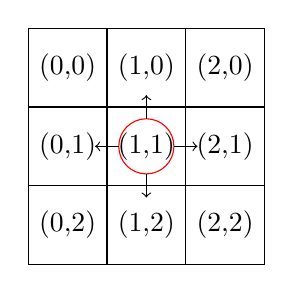
\begin{tikzpicture}[scale=1, auto, swap]
                \foreach \i in {0,1,2} {
                    \foreach \j in {0,1,2} {
                        \node[minimum size=1cm,draw] at (\i,-\j) {(\i,\j)};
                    }
                }
                
                \draw[red] (1,-1) circle (0.35cm);
                
                \draw[->] (1,-0.65) -- (1,-0.35) node[midway, right] {};
                \draw[->] (1.35,-1) -- (1.65,-1) node[midway, above] {};
                \draw[->] (1,-1.35) -- (1,-1.65) node[midway, right] {};
                \draw[->] (0.65,-1) -- (0.35,-1) node[midway, above] {};
            \end{tikzpicture}
            
            \caption{4-Neighbourhood}
            \label{fig:4_neighbourhood}
        \end{column}
        \begin{column}{0.45\textwidth}
            \centering
            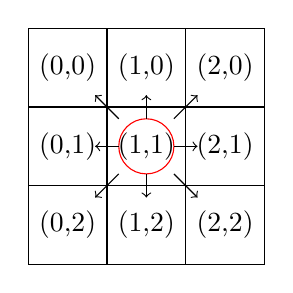
\begin{tikzpicture}[scale=1, auto, swap]
                \foreach \i in {0,1,2} {
                    \foreach \j in {0,1,2} {
                        \node[minimum size=1cm,draw] at (\i,-\j) {(\i,\j)};
                    }
                }
                
                \draw[red] (1,-1) circle (0.35cm);
                
                \draw[->] (1.35,-1) -- (1.65,-1) node[midway, above] {};
                \draw[->] (1.35,-1.35) -- (1.65,-1.65) node[midway, above] {};
                \draw[->] (1,-1.35) -- (1,-1.65) node[midway, right] {};
                \draw[->] (0.65,-1.35) -- (0.35,-1.65) node[midway, above] {};
                \draw[->] (0.65,-1) -- (0.35,-1) node[midway, above] {};
                \draw[->] (0.65,-0.65) -- (0.35,-0.35) node[midway, above] {};
                \draw[->] (1,-0.65) -- (1,-0.35) node[midway, right] {};
                \draw[->] (1.35,-0.65) -- (1.65,-0.35) node[midway, above] {};
            \end{tikzpicture}
            
            \caption{8-Neighbourhood}
            \label{fig:8_neighbourhood}
        \end{column}
    \end{columns}
   
    \label{fig:neighbourhoods}
\end{figure}
\end{frame}

\begin{frame}[t]
\frametitle{Basic Idea of Image Denoising}
\begin{figure}[!ht]
  \centering
  \resizebox{1\textwidth}{!}{
    \begin{tikzpicture}[node distance=3.5cm]
      \node (img1) at (0,2) {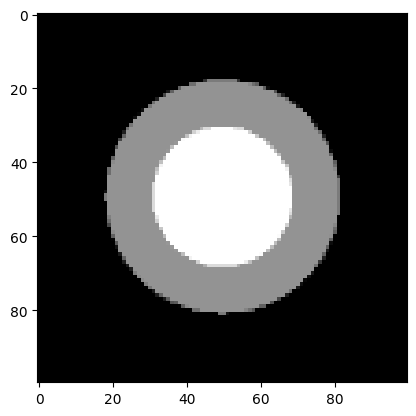
\includegraphics[width=4cm]{img/img.png}};
        \node (plus1) at (0, -1) {$\mathbf{+}$};
      \node (img2) at (0, -4) {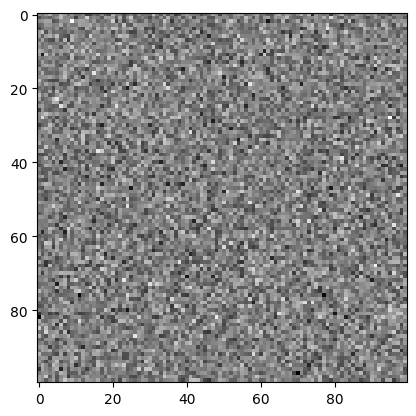
\includegraphics[width=4cm]{img/noise_2.png}};
      
      \node (img3) at (10, 0) {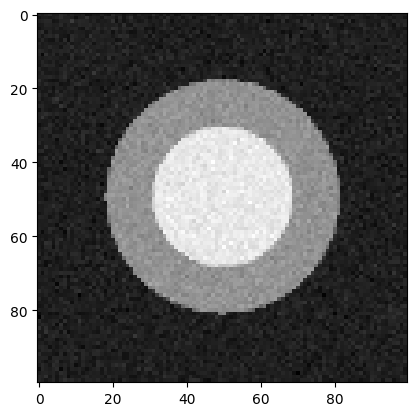
\includegraphics[width=4cm]{img/noisy_im.png}};
      \node (img4) at (18,0) {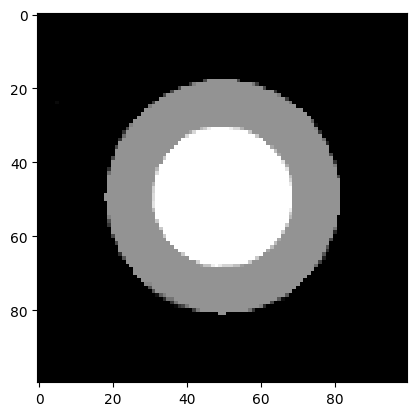
\includegraphics[width=4cm]{img/denoised.png}};

      \draw [->] (img1) -- (img3);
      \draw [->] (img2) -- (img3);
      \draw [->] (img3) -- (img4);
       \node [above] at (img1.north) {Image};
  \node [above] at (img2.north) {Noise};
  \node [above] at (img3.north) {Noise added Image};
  \node [above] at (img4.north) {Denoised Image};
\draw [<->] ([yshift=0.1cm]img1.east) to[out=60, in=120] node[midway, above] {Metrics(example): PSNR, SNR, SSIM} ([yshift=0.8cm]img4.west);
    \end{tikzpicture}
  }
  \caption{Image Denoising}
\end{figure}
\end{frame}

\begin{frame}{Some Basic Denoising filters}
    \begin{block}{Mean Filter}
    Given an input image $I$, we define its pixels at position $(x,y)$  as $I(x,y)$.
For each output pixel  $I'(x,y)$  we find the mean value with a local region R  surrounding $(x,y)$\\ 
$I'(x,y)$ = mean\{$I(x+i,y+j)|(i, j) \in R$\}
    \end{block}
    
    \begin{columns}
        \column{0.5\textwidth}
            \begin{figure}
                \centering
                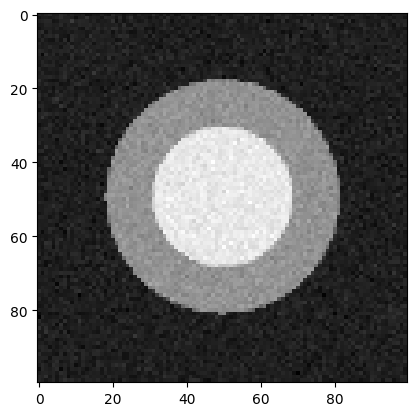
\includegraphics[scale = 0.4]{img/noisy_im.png}
                \caption{Image}
                \label{fig:dual fig demo 1}
            \end{figure}
            
        \column{0.5\textwidth}
        \begin{figure}
            \centering
            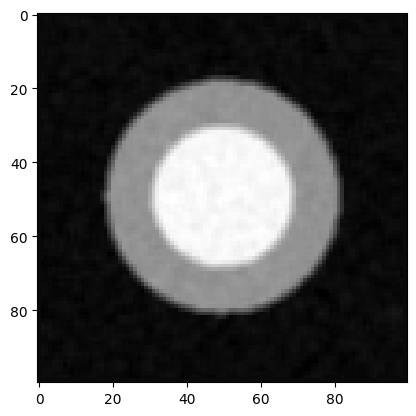
\includegraphics[scale = 0.4]{img/mean.png}
            \caption{After Mean Filter}
            \label{fig:dual fig demo 2}
        \end{figure}
\end{columns} 

\end{frame}
\begin{frame}{Some Basic Denoising filters}
    \begin{block}{Median Filter}
    Given an input image $I$, we define its pixels at position $(x,y)$  as $I(x,y)$.
For each output pixel  $I'(x,y)$  we find the mean value with a local region R  surrounding $(x,y)$\\ 
$I'(x,y)$ = median \{$I(x+i,y+j)|(i, j) \in R$\}
    \end{block}
    
    \begin{columns}
        \column{0.5\textwidth}
            \begin{figure}
                \centering
                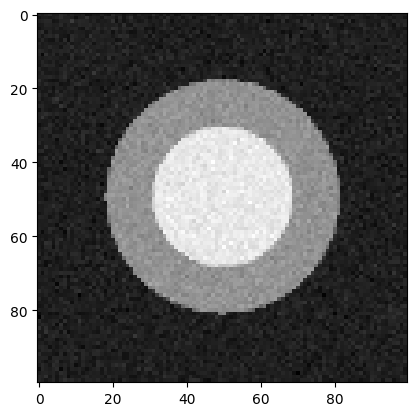
\includegraphics[scale = 0.4]{img/noisy_im.png}
                \caption{Image}
                \label{fig:dual fig demo 1}
            \end{figure}
            
        \column{0.5\textwidth}
        \begin{figure}
            \centering
            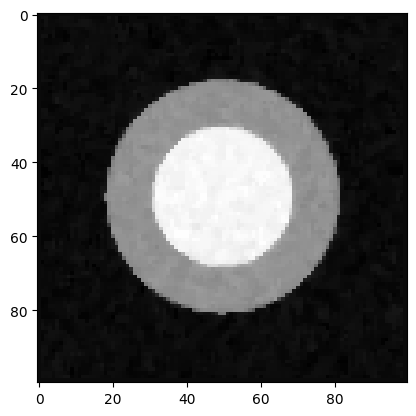
\includegraphics[scale = 0.4]{img/medain.png}
            \caption{After Median Filter}
            \label{fig:dual fig demo 2}
        \end{figure}
\end{columns} 

\end{frame}
\section{Iterative scheme}

\begin{frame}{Some basic Terminology of the paper}
\frametitle{Some basic Terminology of the paper}
    \begin{itemize}
        \item \textbf{Shrinkage Parameter ($\theta$):} The shrinkage parameter, often represented by $\theta$, is used in the shrinkage function $T_{\theta}(u)$ in the iterative scheme. Shrinkage is used to reduce the influence of noise while preserving the essential features of the image.
        \item \textbf{Smoothing Parameter ($\alpha$):}  Smoothing is a process that reduces the local variations in an image, making neighboring pixel intensities more similar. The smoothing parameter, often represented by $\alpha$, is a factor that controls the extent of smoothing applied to the image in each iteration. 
        
    \end{itemize}
\end{frame}

\begin{frame}{The Iterative scheme}
\frametitle{The Iterative scheme}
    \begin{itemize}
        \item Given an observed image $u_0 = (u^0_{i,j}),{i=0,\ldots,N_1-1;j=0,\ldots,N_2-1}$
        
        \item noise $n = (n_{i,j})_{i=0,\ldots,N_1-1;j=0,\ldots,N_2-1}$,  $n$ is Normally-distributed noise $n_{i,j} \in N(0, \sigma^2)$
        
        \item  where $u_0 = f + n$
        \item shrinkage parameter $\theta > 0$ and a smoothing parameter $0 < \alpha \leq \frac{1}{6}$.
        \itemm iteration for $k = 0, 1, \ldots$ For $i = 0, \ldots, N_1 - 1$ and $j = 0, \ldots, N_2 - 1$, compute the new image values as:
	\begin{equation}
		u_{i,j}^{k+1} = u_{i,j}^k + \alpha\sum_{\substack{(l,m)\in N(i,j)\\(l,m)\neq (i,j)}} \frac{T_{\theta}(u_{l,m}^k - u_{i,j}^k)}{(l-i)^2 + (m-j)^2} \label{eq:1}
	\end{equation}
        \item 	Here $T_\theta$ function is defined as 
	$T_{\theta}(x) = \begin{cases}
		0 & \text{if } |x| \geq \theta \\
		x & \text{if } |x| < \theta
	\end{cases}$
    \end{itemize}
\end{frame}


\begin{frame}{The Iterative scheme}
\frametitle{The Iterative scheme}
    \begin{itemize}
       \item 	The neighborhood $ N(i, j)$ is defined as $N(i, j) := \{(l, m) : |i - l| \leq 1; |j - m| \leq 1\}
	$, denotes the set of pixels $(l, m)$ that fall within a $(3\times 3)$ neighborhood centered at pixel $(i, j)$.
	 \item Then we can rewrite it:

\begin{equation}
	u^{k+1}_{i, j} = u^k_{i, j} + \alpha \sum_{\substack{r=-1\\r\neq 0}}^{1}\sum_{\substack{s=-1\\s\neq 0}}^{1} \frac{T_{\theta}(u^k_{i+r,j+s} - u^k_{i, j})}{r^2 + s^2}  \label{eq:2}
\end{equation}

	
    \end{itemize}
\end{frame}
\begin{frame}[plain]
Let us now consider the properties and convergence of the iteration scheme. For convenience, we restrict our considerations to the scheme (2). All ideas can be simply transferred to more complex schemes.

We choose one index for pixel numbering of the digital image $u^k$. Put $N := N_1 \cdot N_2$ and
$n = i + N_1j$, $i = 0, \ldots, N_1 - 1$, $j = 0, \ldots, N_2 - 1$,
such that the pixel $n$ corresponds to $(i, j)$. Then the iteration scheme (2) can be written in matrix-vector form as
$u^{k+1} = A^k u^k$,
where $u^k = (u^k_0, \ldots, u^k_{N-1})^T$ and where $A^k = (A^k_{n,p})_{N \times N}$ is a sparse matrix of the form
\[
A^k_{n,p} :=
\begin{cases}
1 - \kappa_n \alpha & \text{for } p = n, \\
\alpha & \text{for } p \equiv \{n - 1, n + 1, n - N_1, n + N_1\} \pmod{N} \\
& \quad \text{and } |u^k_n - u^k_p| < \theta, \\
\alpha/2 & \text{for } p \equiv \\ & \{n - 1 + N_1, n + 1 + N_1, n + 1 - N_1, n-1-N_1\}\\& \pmod{N} 
 \quad \text{and } |u^k_n - u^k_p| < \theta, \\
0 & \text{elsewhere}.
\end{cases}
\]

\end{frame}

\begin{frame}[plain]
Let's $u^1$ = \begin{bmatrix}
96 & 182 & 45 \\
199 & 184 & 162 \\
138 & 212 & 201 \\
\end{bmatrix}.\\

Then after apply the conditions, A^1=\\

\resizebox{\textwidth}{!}{%
$\begin{bmatrix}
1 & 0 & 0 & 0 & 0 & 0 & 0 & 0 & 0 \\
0 & 1-\frac{3\alpha}{2} & 0 & \frac{\alpha}{2} & \alpha & \frac{\alpha}{2} & 0 & 0 & \frac{\alpha}{2} \\
0 & 0 & 1 & 0 & 0 & 0 & 0 & 0 & 0 \\
0 & \frac{\alpha}{2} & 0 & 1-\frac{3\alpha}{2} & \alpha & 0 & 0 & \frac{\alpha}{2} & \frac{\alpha}{2} \\
0 & \alpha & 0 & \alpha & 1-\frac{9\alpha}{2} & \alpha & 0 & \alpha & \frac{\alpha}{2} \\
0 & \frac{\alpha}{2} & 0 & 0 & \alpha &1-2\alpha & \frac{\alpha}{2} & 0 & 0 \\
0 & 0 & 0 & 0 & 0 & \frac{\alpha}{2} & 1-\frac{\alpha}{2} & 0 & 0 \\
0 & 0 & 0 & \frac{\alpha}{2} & \alpha & 0 & 0 & 1-\frac{3\alpha}{2} & \alpha \\
0 & \frac{\alpha}{2} & 0 & \frac{\alpha}{2} & \frac{\alpha}{2} & 0 & 0 & \alpha & 1-\frac{3\alpha}{2} \\
\end{bmatrix}$.%
}
\end{frame}

\begin{frame}[plain]
Here $\kappa_n$ (with $0 \leq \kappa_n \leq 6$) is chosen such that the sum of entries in the $n$th row of $A^k$ is 1.
Now we observe the following properties of the iteration matrix $A^k$.
\begin{enumerate}
    \item The number of nonzero entries in each row (column) of $A^k$ is at most 9.
    \item For $\alpha \leq \frac{1}{6}$, all entries of $A^k$ are non-negative, i.e., $A^k \geq 0$.
    \item With $1 := (1, \ldots, 1)^T \in \mathbb{R}^N$, we have $A^k 1 = 1$.
    \item The iteration matrix $A^k$ is symmetric, i.e., $A^k = (A^k)^T$.
\end{enumerate}

\end{frame}


\begin{frame}[plain]
\begin{itemize}
    \item By suitable ordering of rows and columns of $A^k$, we can transfer $A^k$ into a block diagonal matrix, where the $n$th and the $p$th row (column) belong to the same block if there exists a sequence of indices $n_1, n_2, \ldots, n_{\nu}$ such that $n_1 \in N(n), n_2 \in N(n_1), \ldots, p \in N(n_{\nu})$ and if $|u^k_n - u^k_{n_1}| < \theta, |u^k_{n_1} - u^k_{n_2}| < \theta, \ldots, |u^k_{n_{\nu}} - u^k_p| < \theta$ holds. 
    
    \item The ordering of $A^k$ into blocks defines a partition $S^k$ of the pixel set $\{0, \ldots, N - 1\}$ into different sets, $S^k = \{S^{k}_m\}_{j=1}^{J^k}$, separating pixels whose pixel values differ strongly enough. Two pixels $n, n'$ are in the same set $S^{k}_m$ if, in the above procedure, the $n$th and the $n'$th row of $A^k$ are transferred into the same block matrix $A^k_m$.
\end{itemize}

\end{frame}


\begin{frame}[plain]

    \begin{itemize}
        \item Let's consider this example($0< \epsilon < \theta$): \[
\begin{pmatrix}
0 & \theta + \epsilon & \theta + \epsilon & \theta + \epsilon \\
0 & \theta + \epsilon & 2\epsilon & \theta + \epsilon \\
0 & \theta + \epsilon & \theta + \epsilon & \theta + \epsilon \\
0 & 0 & 0 & 0 \\
\end{pmatrix}
\]
Partition/Block positions:$\{\{0, 4, 8, 12, 13, 14, 15\}, \{1, 2, 3, 5, 6, 7, 9, 10, 11\}\} $
Considering elements positions like- $0$^{th} =$0$, $1$^{st}= $\theta + \epsilon$ ....so on
    \end{itemize}
\end{frame}

\begin{frame}[plain]

    \begin{itemize}
        \item  Let's consider a new example:  
        \[ u^0= 
\begin{bmatrix}
96 & 120 & 100 \\
70 & 180 & 140 \\
50 & 100 & 180 \\
\end{bmatrix}
\]
Blocks coordinate: 3 \[[ (0, 0), (2, 1), (0, 2), (0, 1), (1, 2)], [(1, 0), (2, 0)], [(1, 1), (2, 2)]\]
\item \[ u^1 = u^{k}=
\begin{bmatrix}
100 & 100 & 100 \\
56 & 180 & 138 \\
56 & 100 & 180 \\
\end{bmatrix}
\]
Blocks coordinate: 4 \[[ (0, 0), (2, 1), (0, 2), (0, 1)], [(1, 0), (2, 0)], [(1, 1), (2, 2)], [(1, 2)]\]
    \item Taking means per block and updating it doesn't change pixels further. 
    \end{itemize}
\end{frame}

\begin{frame}[plain]
Let $S^k = \{S^{k}_m\}_{m=1}^{J^k}$ be the partition of the pixel set,
Now let us consider the new partition $S^{k+1}$ is different from $S^k$, then for a fixed set $S^{k}_m \in S^k$, the following types of changes are possible:

\begin{enumerate}
    \item $S^{k}_m$ is divided into two or more subsets $S^{k+1}_{m1}, S^{k+1}_{m2}, \ldots$.
    \item $S^{k}_m$ is united with one or more neighboring sets, i.e., $S^{k+1}_{m1} = S^{k}_m \cup S^{k}_m' \cup \ldots \cup S^{k}_m\nu$.
    \item $S^{k}_m$ is united with one or more neighboring subsets of $S^{k}_m'$ to obtain a new set $S^{k+1}_{m1}$ of $S^{k+1}$.
    \item $S^{k}_m$ is divided into two or more subsets $S^{k+1}_{m1}, \ldots$ which are themselves united with one or more neighboring sets $S^{k}_m'$ (or neighboring subsets of $S^{k}_m'$).
\end{enumerate}
\begin{itemize}
    \item let
\begin{equation}
    \mu^k_{m} = \frac{1}{\#S^{k}_m} \sum_{n \in S^{k}_m} u^k_{n}, \quad m = 1, \ldots, J_k  \label{eq: 3}
\end{equation}

 {\#S^{k}_m}\text{ denotes number of the elements on a block.}
\end{itemize}
\end{frame}

\begin{frame}[plain]
  \begin{block}{Theorem}
    Now let's consider a noisy image $u^0$. The iteration scheme (\ref{eq:2}) with $\alpha \leq \frac{1}{6}$ and starting with the noisy image $u^0$. Then, after a finite number of $k$ iterations, the partition $S_k = (S_{m}^{k})^{j_k}_{m=1}$ of pixels corresponding to the blocks $A_{m}^{k},\ m = 1, \ldots, J_k$ of the ordered iteration matrix $A_k$ is settled and will not change further, i.e., there exists a finite $k$ such that $S^k = S^{k+\nu},\ \nu = 1, 2, \ldots$.

The iteration scheme (\ref{eq:2}) will converge to the spatial average of $u^k$ in all subsets $S^k_m$:

\[
\lim_{{\nu \to \infty}} u^{k+\nu} =  \sum_{{m=1}}^{{J_k}} \mu^{k}_m \chi_{S^k_m}
\]

where $ \mu^{k}_m$ is in (\ref{eq: 3}) and where $\chi_{S^k_m}$ is the characteristic function corresponding to the index set $S^k_m$, i.e.,

\[
\chi_{S^k_m}(n) =
\begin{cases}
	1 & \text{if } n \in S_{m}^{k} \\
	0 & \text{if } n \notin S_{m}^{k}
\end{cases}
\]
    \end{block}


\end{frame}
\section{Algorithm and hints on implementation}
\begin{frame}{Algorithm}
\begin{block}{Algorithm for Denoising Piecewise Constant Images}
    

The complete algorithm for denoising piecewise constant images consists of three steps. Let $u^0 = (u^0_{i,j})_{i=1}^{N_1 -1},j_{i=1}^{N_2-1}$ be the given noisy image.
\begin{enumerate}
    \item For a fixed thresholding parameter $\theta > 0$, a smoothing parameter $\alpha \leq \frac{1}{6}$, and a fixed number $K \in \mathbb{N}$, perform the iteration:

\[
u^{k+1}_{i,j} = u^k_{i,j} + \alpha \sum_{\substack{r,s=-1 \\ \ (r,s) \neq (0,0)}}^{1} \frac{T_{\theta}(u^k_{i+r,j+s} - u^k_{i,j})}{r^2 + s^2}
\]

for $k = 0, 1, 2, \ldots, K-1$, using periodic boundary conditions

\end{enumerate}
\end{block}
  
\end{frame}
\begin{frame}{Algorithm}
\begin{block}{Algorithm for Denoising Piecewise Constant Images}
    

\begin{enumerate}
    \item[2.] Apply the following mean value procedure. Establish a new iteration matrix $A_K$  with a suitable shrinkage parameter $\theta_1$. Take the partition $(S^K_m)^{J_K}_{m=1}$ determined by this iteration matrix $A_K$. Compute for $m = 1, \ldots, J_K$ the mean values:

\[
\mu^K_m = \frac{1}{{\#S^K_m}} \sum_{n \in S^K_m} u^K_n
\]

Replace each value $u^K_n$ with $n \in S^K_m$ by $\mu^K_m$.

\end{enumerate}
\end{block}
  
\end{frame}


\begin{frame}{Algorithm}
\begin{block}{Algorithm for Denoising Piecewise Constant Images}
    

\begin{enumerate}
    \item[3.] Using the partition $(S^K_m)^{J_K}_{m=1}$, apply the following median value procedure. All pixel values belonging to subsets of the partition with less than 6 components are replaced by the median of their neighbor pixel values.

\end{enumerate}
\end{block}
  
\end{frame}


\begin{frame}[plain]
\begin{block}{Methodology}
    
\end{block}
\begin{figure}
    \centering
    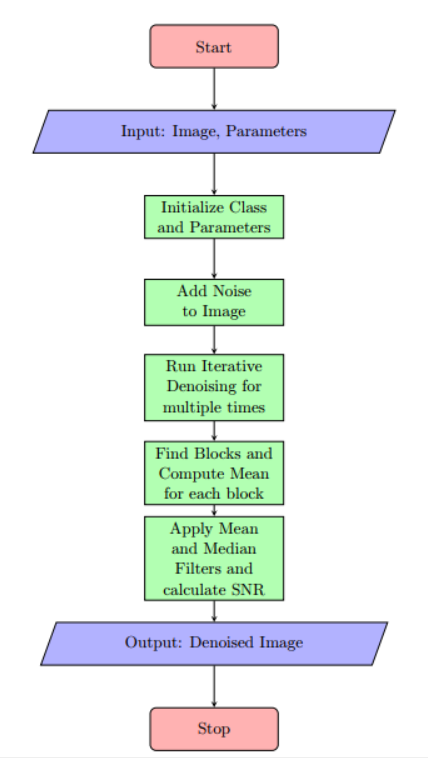
\includegraphics[scale = 0.35]{img/method.png}
    \caption{Flowchart of the Plonka-Hoch and Jianwei Ma Denoising Process}
    \label{fig:fig demo}
\end{figure}


\end{frame}
\section{Performance}

\begin{frame}{Some Considerations}

    \begin{itemize}
        \item the following equation has been used for calculating ``Signal-to-noise ratio''. 
	\begin{equation}
		\text{SNR} = 20 \log_{10} \frac{\| \mathbf{f} - \bar{\mathbf{f}} \|}{\| \mathbf{n} \|}
	\end{equation}
	
	\item For finding good starting points for shrinkage parameters for the denoising process (theoretically), determining  contrast ``c'' in an image which is the difference between the maximum and minimum pixel intensity is necessary. It quantifies how much the intensity varies across the image, with higher values indicating more variation. ``c'' is defined as - 
	\begin{equation}
		c = \min\left\{\left|f_{i,j} - f_{i',j'}\right|, (i', j') \in N(i, j), f_{i,j} \neq f(i', j')\right\}
	\end{equation}

    \end{itemize}
\end{frame}

\begin{frame}{Some Considerations}

    \begin{itemize}
     \item For small contrast-to-noise ratio i.e. $\frac{c}{\sigma} \leq 1.5$, initiate the iteration process (\ref{eq:2}) with $\theta = \infty$. 
     
     \item The smoothing parameter $\alpha$ need not be chosen very small. An $\alpha$ value in the range of $\left[\frac{1}{10}, \frac{1}{6}\right]$ provides quick smoothing while preserving the convergence result.
     
     \item The optimal number of iterations $K$ is image-dependent and varies with the signal-to-noise ratio. 
		\item If the partition process isn't complete after the first step, paper recommends to use a new shrinkage parameter $\theta_{1} =\frac{\theta c}{10\sigma} $ (see page no. $15$).

    \end{itemize}
\end{frame}
\begin{frame}{Results}

    \begin{itemize}
     \item Image with good contrast-to-noise ratio: $\theta = 30$, $\theta_1 = 4 $
     \begin{figure}[h] % Use [H] instead of [h]
	
		\centering
		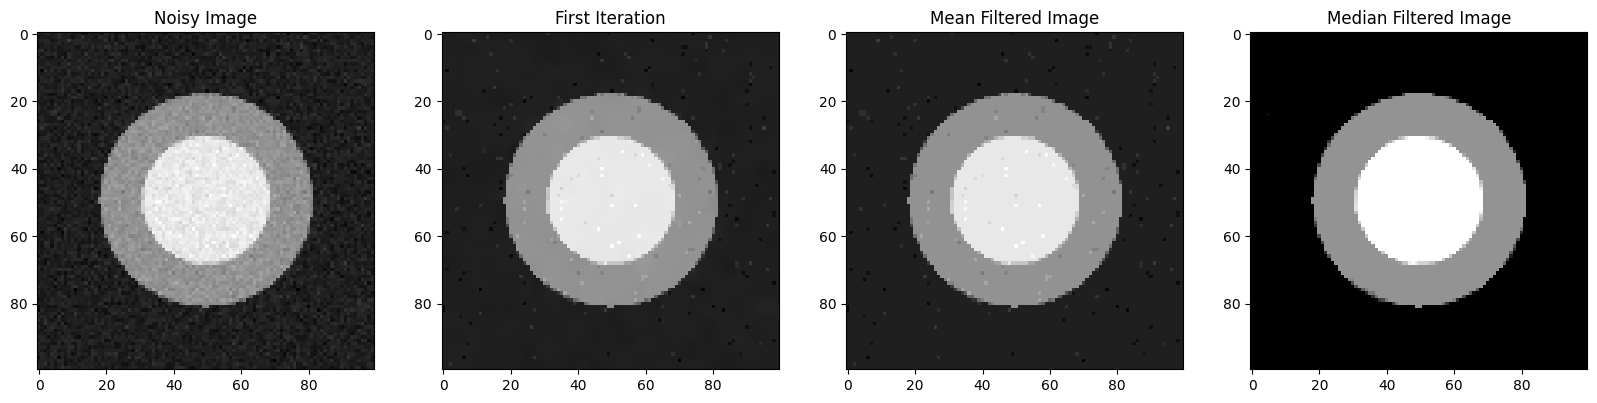
\includegraphics[width=1\linewidth]{img/output.png}
		\caption{Denoising image with different gray level}
		\label{fig:Denoising image with different gray level}
\end{figure}%
    \end{itemize}
\end{frame}

\begin{frame}{Results}

    \begin{itemize}
\item  Influence of the shrinkage parameter on an image with a good contrast-to-noise ratio: $\theta = 40$, $\theta_1 = 40$
\begin{figure}[h] % Use [H] instead of [h]

	
	\centering
	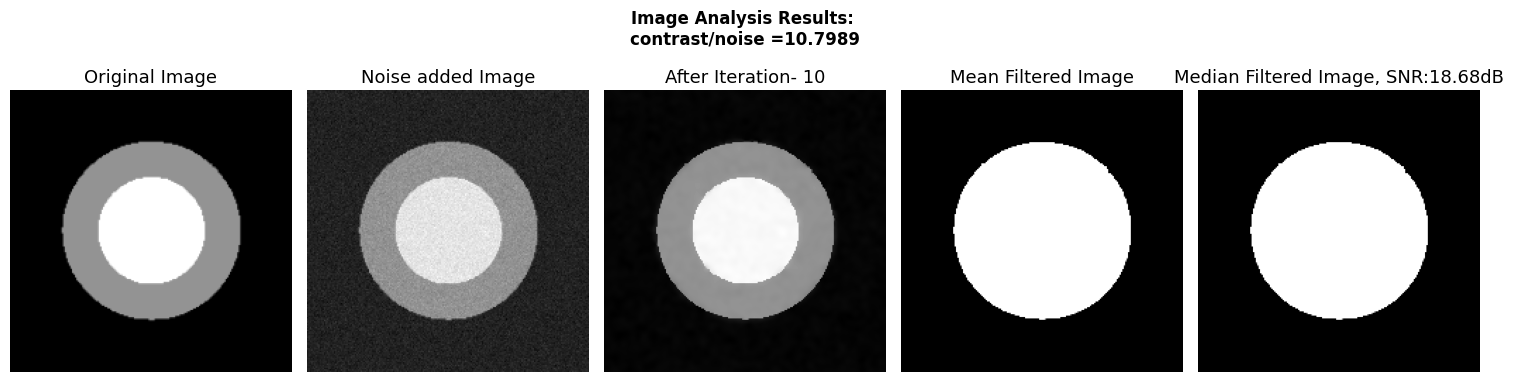
\includegraphics[width=1\linewidth]{img/theta_e.png}
	\caption{Denoising image with different gray level - Shrinkage parameter influence}
	\label{fig: Denoising image Theta influence}
\end{figure}
    \end{itemize}
\end{frame}


\begin{frame}{Results}

    \begin{itemize}

\item Example for small contrast-to-noise ratio image:  $\frac{c}{\sigma}<1.5 $ and $\theta = \infty$,  $\theta_1 = 4$

\begin{figure}[h] % Use [H] instead of [h]
	\centering

	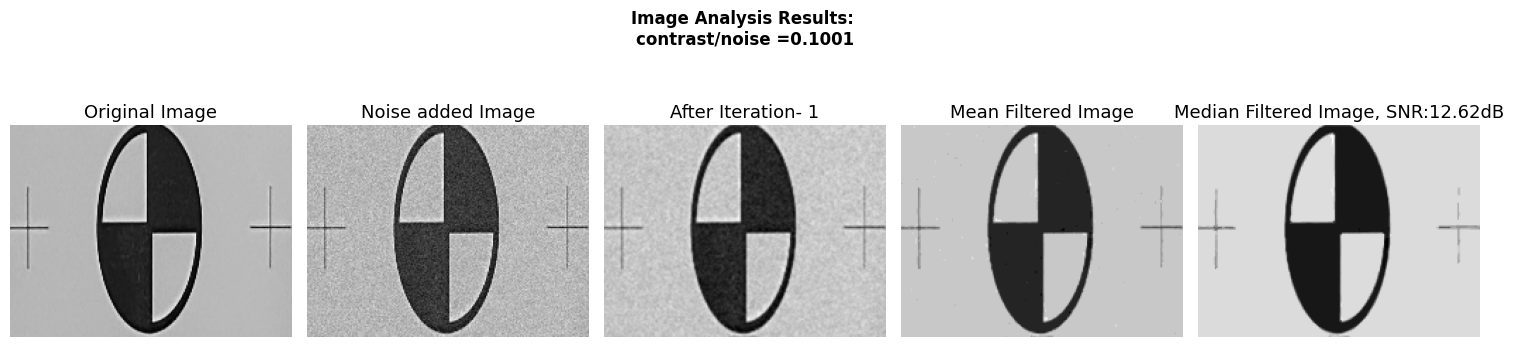
\includegraphics[width=1\linewidth]{img/hardone.png}
	\caption{Denoising image with different gray level - low contrast-to-noise ratio }
	\label{fig: low contrast-to-noise ratio}
\end{figure}

    \end{itemize}
\end{frame}


\begin{frame}{Results}

    \begin{itemize}
\item Here is another example of a small contrast-to-noise ratio image:  $\frac{c}{\sigma}<1.5 $ and $\theta = \infty$, $\theta_1 = 6$

\begin{figure}[h] % Use [H] instead of [h]
	\centering
	
	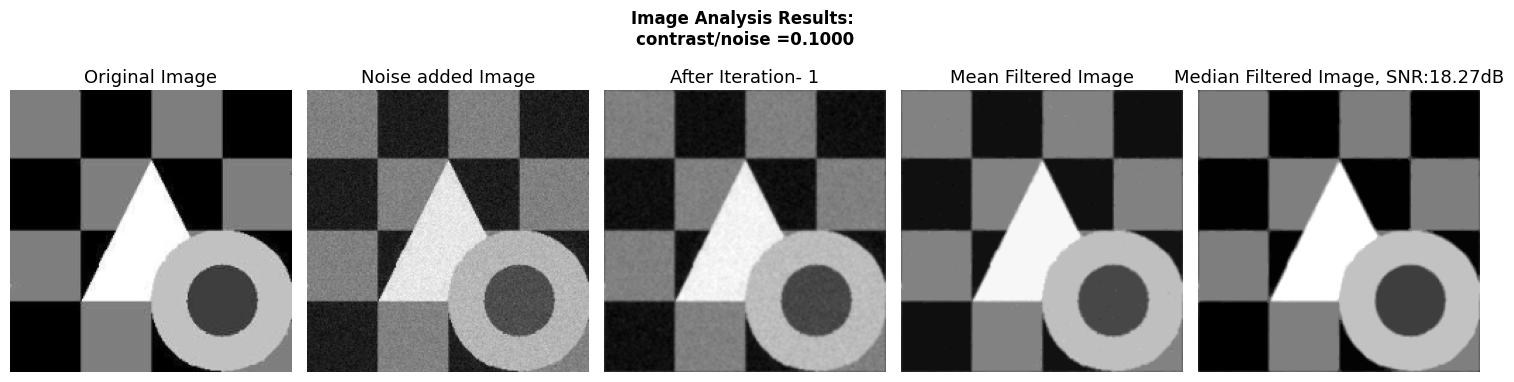
\includegraphics[width=1\linewidth]{img/hardone_2.png}
	\caption{Denoising image with multiple gray level - low contrast-to-noise ratio }
	\label{fig: low contrast-to-noise ratio 2}
\end{figure}

    \end{itemize}
\end{frame}

\begin{frame}{Results}

    \begin{itemize}
\item  Does an increase in the number of iterations lead to significantly improved denoising results? This is something we will examine closely. In tandem, we'll also monitor the evolution of block sizes.  
	
	\begin{figure}[H] % Use [H] instead of [h]
		\centering
		
		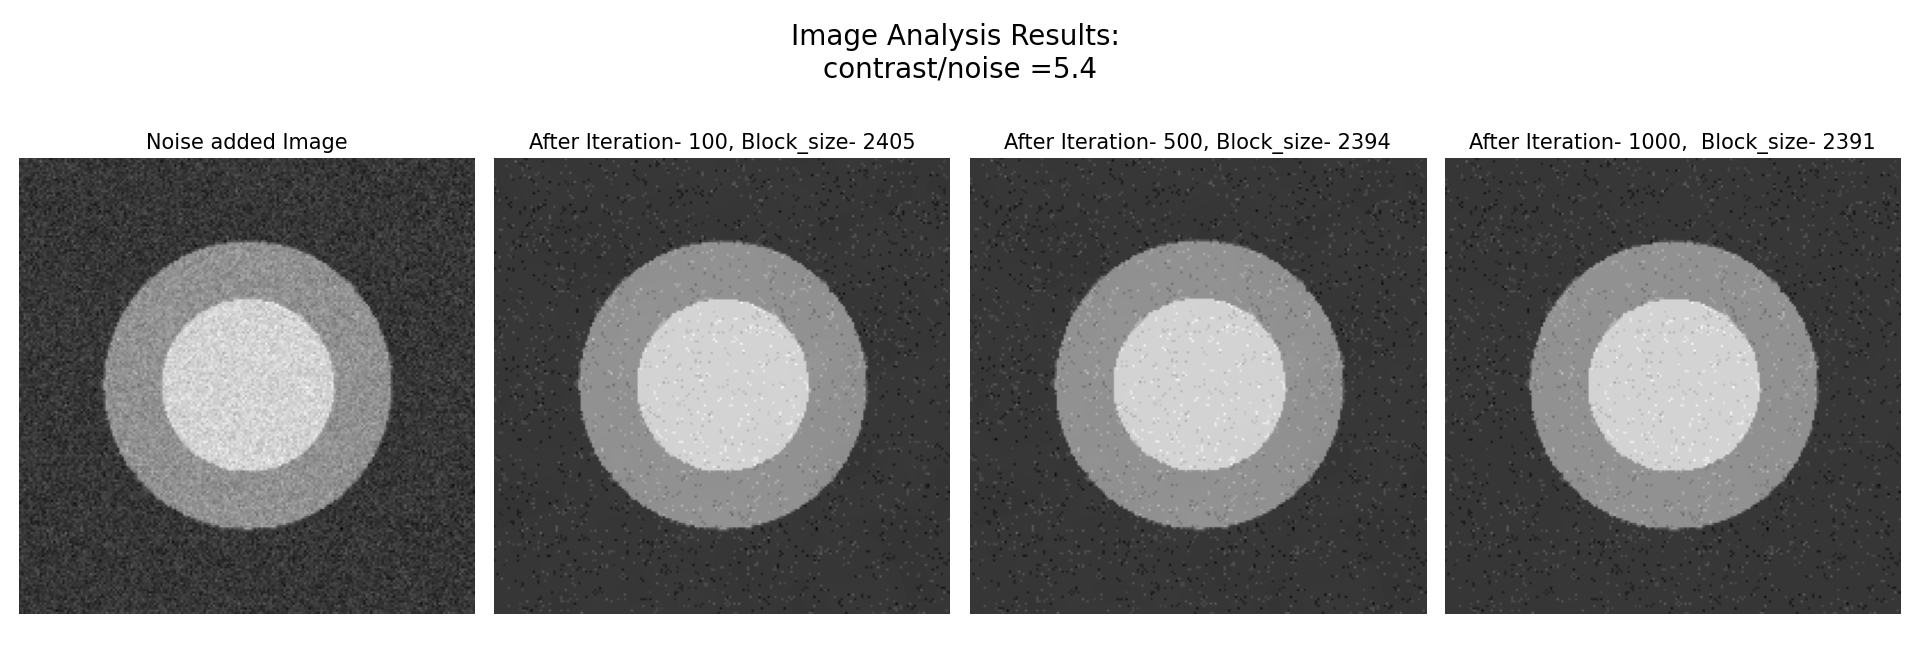
\includegraphics[width=1\linewidth]{img/block.png}
		\caption{Denoising image with multiple gray level - after $100,500,1000$ iteration  }
		\label{fig: after $100,500,1000$ iteration }
	\end{figure}

    \end{itemize}
\end{frame}

\begin{frame}{Applications}

    \begin{itemize}
		\item  In medical imaging, such as MRI or CT scans, noise reduction is crucial for accurate diagnosis.  One of such example can be found here \cite{ongie2016off}.
		
		\item Images captured by remote sensing satellites or aerial drones often suffer from noise due to atmospheric conditions or sensor limitations. 
		
		\item  In industries such as manufacturing or quality control, image denoising is essential for accurate defect detection and inspection. 
		
		\item In Fingerprint Denoising algorithm can highlight these features by reducing the noise within each region.
    \end{itemize}
\end{frame}




%% Final page
\begin{frame}[plain]
    \begin{picture}(0,0)        
        \put(-116, -155){
\includegraphics[width=1.01\paperwidth]{src/title_bg_copy.png}}
        \put(-95, 61){
\includegraphics[width=0.18\paperwidth]{src/goettingen.png}}
    \end{picture}
    \centering\usebeamerfont{acknowledgement}\usebeamercolor[fg]{acknowledgement}\textcolor{main}{Thank You!}
\end{frame}

%% Bibliography
\appendix
\begin{frame}[allowframebreaks]{References}
    \printbibliography
\end{frame}
\end{document}